\documentclass[11pt,a4paper]{cepcnote}
\graphicspath{{figures/}}
\usepackage{cepcphysics}
\usepackage{subfigure}
\usepackage{mathrsfs}
\usepackage{authblk}
\usepackage{textcomp}

\newcommand{\pho}{\phantom{0}}
\newcommand{\bslash}{\ensuremath{\backslash}}
\newcommand{\BibTeX}{{\sc Bib\TeX}}

%\newcommand{\gg}{\gamma\gamma}
\newcommand{\Zqq}{Z\rightarrow q\bar q}
\newcommand{\PRZH}{\sigma(ZH)}
\newcommand{\qt}{\PRZH\cdot BR(\Hgg)\cdot BR(\Zqq)}
\newcommand{\prcs}{\epem\rightarrow ZH\rightarrow q \bar q\gamma\gamma}
%\newcommand{\epem}{e^+e^-}

\title{Measurement of $BR(\Hgg)$ via $\Zqq$ channel in $\epem$ collider at 250 GeV}
\author{The CEPC Collaboration}
%\cepcnote{CEPC\_ANA\_HIG\_2015\_XXX}
\abstracttext{We examine the prospects of measuring $BR(\Hgg)$ with a 125 GeV Higgs boson by measuring the cross section of the process $\prcs$ at the future Circular Electron Positron Collider (CEPC), assuming a integrated luminosity of $5\text{ab}^{-1}$ at center-of-mass energy of 250 GeV. Full simulations with the current CEPC model (CEPCv1) are used to determine the efficiency and shape of the signal and background data, and Monte Carlo (MC) simulations are used to determine the uncertainty of the measurement. A relative uncertainty of 15.6\% can be achieved for the measurement of $\qt$. The uncertainty's dependence on the photon reconstruction efficiency and calorimeter performance is also studied.}

\begin{document}
%\tableofcontents
%\clearpage

\section{Introduction}
In 2012, the ATLAS and CMS Collaborations discovered a 125 GeV boson consistent with the standard model Higgs boson \cite{Aad:2012tfa, Chatrchyan:2012xdj}. %add: "consistent" part cite see Feng
To fully understand the fundamental couplings associated with the Higgs boson, more precision measurement has to be made in future $\epem$ colliders \cite{Accomando:1997wt}. As the Higgs boson is regarded as a portal to new physics beyond standard model, it is important to carefully compare the Higgs couplings to standard model predictions. The measurement of the Higgs di-photon branching ratio $BR(\Hgg)$ is an interesting candidate for this purpose, since not only does the process have a clean final state topology, but it may also contain loop contributions from new charged particles.
However, the fact that this process is mediated by a particle loop causes the branching ratio to be relatively small. At Higgs mass $M_H=125$ GeV, it reaches the maximum of about 0.23\%\cite{Actis:2008ts}.

In this paper we study an important channel involved in the total measurement of $BR(\Hgg)$, the $Z$ boson di-jet decay channel in the Higgsstrahlung process, namely, $\epem\rightarrow ZH\rightarrow q\bar q\gamma\gamma$. Analysis is performed based on full simulation using the detector model CEPCv1 described in section \ref{sec:sim}, making this study compliment to \cite{Feng:MC}. We assume a 125 GeV Higgs boson, with 250 GeV center-of-mass energy collision of integrated luminosity of $5\text{ab}^{-1}$. The statistical precision of the measurement is determined by first casting the fully-simulated and reconstructed signal and background event in the (Higgs-decayed) di-photon invariant mass space and then performing Monte Carlo simulations based on the distribution to obtain the uncertainty of the measurement. We may also obtain uncertainty of the uncertainty reported by the fit program in signal fitting with multiple runs. Alternatively, one can use event counting $S/\sqrt{S+B}$ as a gauge for precision, where $S$ and $B$, respectively, are the number of signal and background events in a small region around the signal peak ($\sim1\sigma$) in the di-photon invariant mass space. The event counting measure is a good indicator of the final uncertainty (from MC simulations), and is used to optimize event selection scheme since it is much faster to evaluate.
The methods used in this study can be easily generalized to the measurement of $BR(\Hgg)$ via other channels such as $\epem\rightarrow ZH\rightarrow \mu\bar\mu\gamma\gamma$, as the analysis relies heavily on the Higgs-decayed di-photon information.

The paper is organized as follows: In section \ref{sec:sig&bkg} we discuss the signal and relevant background processes and their theoretical detector responses. In section \ref{sec:sim} we describe the CEPCv1 detector model used in simulation (and the reconstruction algorithm). In section \ref{sec:measurement} we present the event selection scheme and the determination of the uncertainty of the $\qt$ measurement. In section \ref{sec:photonrec} we further study the relation between the photon reconstruction algorithm and the measurement uncertainty. 
%We reserve section \ref{sec:conclusion} for our conclusion.

\section{Signal and background}
\label{sec:sig&bkg}
In $\epem$ collision, the Higgs boson can be produced via Higgsstrahlung $\epem\rightarrow ZH$, and the $W$ or $Z$ boson fusion $\epem\rightarrow \nu_e\bar\nu_eH$ and $\epem\rightarrow\epem H$ \cite{Glashow:1961tr,Weinberg:1967tq,salam1968elementary}. At $\sqrt{s}=250$ GeV and $M_H=125$ GeV, the Higgsstrahlung process has a cross section of approximately 200 fb, much larger than the $W$ and $Z$ fusion production of the Higgs. Moreover, the hadronic decay of the $Z$ boson also has a high branching ratio of about 70\% in this energy level, thus the process $\epem\rightarrow ZH\rightarrow q\bar q\gamma\gamma$ consists a major part of the processes involved in measuring $BR(H\rightarrow\gamma\gamma)$. Assuming $BR(H\rightarrow\gamma\gamma)=0.23\%$, and an integrated luminosity of $5000fb^{-1}$ in 10 years of data taking in CEPC, we expect in total of approximately 1633 signal events.

The general tree-level background for $\epem\rightarrow q\bar q\gamma\gamma$ consists of quark pair productions via photon and $Z$ boson, with additional photons coming from initial state radiations (ISR) and final state radiations (FSR). The relevant diagrams agrees with the diagrams listed in \cite{Boos:2000bz}. The reducible background processes in which the quarks are produced via photon will be essentially eliminated using invariant mass information and our event selection scheme, and so are processes with no ISR since the $Z$ boson would be significantly off-shell. Otherwise, two energetic ISR photons or one ISR and one FSR photon may mimic the Higgs-decayed photons, while the quark pair also comes from an on-shell $Z$ boson. We shall therefore ignore the reducible background events and focus on irreducible background where the photons mimics decay products of a particle recoiled by the on-shell $Z$ boson.

The Monte Carlo data used for signal and background events are generated by the Whizard 1.95 package \cite{Kilian:2007gr}. Due to the enormous amount of background events with low energy photons that can be easily eliminated in event selection, a pre-selection is performed on the MC sample before being taken to full simulation:
\begin{itemize}
\item The two most energetic photons with $\cos\theta_\gamma < 0.99$ must both exceed 25 GeV in energy. ($\theta_\gamma$ is the polar angle.)
\item The two photons must satisfy $(\cos\theta_{\gamma_1}+1)(\cos\theta_{\gamma_2}-1) < -0.05$ and $(\cos\theta_{\gamma_1}-1)(\cos\theta_{\gamma_2}+1) < -0.05$
\item The invariant mass of the two photons must satisfy $100\GeV<M_{\gamma\gamma}<160\GeV$
\end{itemize}
The pre-selection imposed here are roughly on the same variables as the event selection imposed later to avoid unexpected deficiencies. To make sure that no events excluded in the pre-selection may enter the final cut in a full simulation due to calorimeter uncertainties, the final event selection boundaries must be more than 3$\sigma$ away from the pre-selection bounds, where $\sigma$ is the uncertainty introduced in the full simulation (principally from calorimeter) on the interested variable. Specifically, the standard deviation of the momentum direction of reconstructed photons is less than 0.0004 rad so that the uncertainty of $(\cos\theta_{\gamma_1}\pm1)(\cos\theta_{\gamma_2}\pm1)$ is about $0.0008\oplus0.0008\approx0.0012$. The uncertainty of $M_{\gamma\gamma}$ is at most (for 160 GeV) $2.0\oplus2.0\approx2.9\GeV$ for Ecal performance of relative uncertainty $16\%/\sqrt{E}$. The first pre-selection is just to ensure that selected area has 100\% Ecal coverage. To reflect the step-wise efficiency of the event selection, another "fast simulated" background sample is produced by imposing only the first of the three pre-selection criteria and then adding a smear to the photon energies to reflect the Ecal uncertainty, with the total efficiency is then adjusted to match the full simulated sample. This "fast simulation" sample is only used in evaluating the efficiency of the event selection. 

%[\textbf{???}:There seems to be no fast way to evaluate the photon reconstruction algorithm's effect on the background except doing no precuts at all.]
%Note that lower energy photons are kept in reconstruction because they may come from the hadron showers and will be used in later analysis.

\section{Simulation and reconstruction}
\label{sec:sim}
\subsection{General simulation and reconstruction}
[Generation: Whizard 1.95. Simulation: Mokka. Reconstruction: ArborV3KD. Detector Geometry: CEPCv1(?)]
[The low-end resolution of Ecal is reflected by discarding all photons with energy less than 1 GeV. (Other low energy photons useful in photon recovery.)]

\subsection{Photon recovery}
Conversion of high energy photons that decayed from Higgs bosons into fermion pairs before reaching the detector is a serious reduction to the reconstructed event number. The general reconstruction algorithm, is not specifically designed for the $ZH\rightarrow q\bar q\gamma\gamma$ process that involves complex environment such as particle showers. It is necessary to develop a photon recovery algorithm specific for this study.

The general reconstruction yields a reconstruction rate of approximately 90\% for photons decayed from Higgs boson in signal events. This means 80\% of the events have both photons coming from the Higgs reconstructed, while another 19\% of the events has one photon recovered.
%(The criterion for a successful reconstruction is shown in a figure \ref{fig:???} in the appendix.)
Since the majority of missing photon is due to conversion into $\epem$ pairs, we need to identify $\epem$ pairs that are close to each other (small track distance) that are consistent with a high energy photon. Partially motivated by the photon recovery algorithm used in \cite{Boos:2000bz}, the following criteria for recovering a pair of electron is adopted:

For all pairs of particles with opposite charges:
\begin{itemize}
\item The angle between the 3 momentums of the particle pair should be less than 19\textdegree.
\item The invariant mass of the particle pair should be less than 5 GeV.
\item There should not be any other visible particles within the 7\textdegree cone of the converted photon's momentum (total of the particle pair).
\end{itemize}
(Selecting all charged particles as electron/positron candidate is due to the relatively large electron pion mistag rate in presence of jets.) The angle of between the 3-momentum is allowing since this criterion does not affect the recovery by much. The third criterion is for preventing false identification, especially from the particle shower. Although it may sacrifice some signal event whose Higgs-decayed photons happens to line up with some hadron debris, the false positive rate of the recovery algorithm is kept low by the final criterion.

After applying the recovery algorithm, the reconstruction rate of a single photon is boosted to $>95\%$, with the success rate for reconstruction of both photons about 92.5\%. We shall assume this recovery rate in the following analysis. The measurement uncertainty's dependence on the recovery rate is studied later in section \ref{sec:photonrec}.

\section{Measurement of $\qt$}
\label{sec:measurement}
\subsection{Event selection}
The measurement of $\PRZH BR(\Hgg) BR(\Zqq)$ is based on the invariant mass information of the two energetic photons presumably decayed from the Higgs boson. We first select two photons with the highest invariant mass from a reconstructed event (after the additional photon recovery), and then apply a series of cut to filter out unwanted backgrounds. In limited Ecal precision, the di-photon momentum information proves to be more useful than the jet information from the quarks with more calorimeter hits, despite the latter's use in filtering out reducible background.

The variables being used in the event selection is selected by the following guideline. In $\prcs$ If we force the Higgs boson to be on-shell, the dip-photon system of the signal events has exactly one degree of freedom less than the irreducible background's because of this additional on shell requirement. However, it is important not to exploit this different in event selection since it would cause the background to mimic the signal in the di-photon invariance mass space. We should look for variables related to the external geometry (e.g. the $z$ axis) where background events have different concentration from the signal events. The polar angles is a good choice since the ISR concentrate around the $z$ axis. Taking into account that the two energetic ISRs are likely to be in opposite directions, a two dimension cut is necessary. We then apply cuts on the angle of the two photons with the recoil momentum to further filter background events based on the paraxial feature of the ISR. We finally apply a two dimensional cut on the energy-invariant mass plane of the di-photon system to single out the signal peak in the invariant mass space. After selecting the cut schemes, we then optimized the parameters using Monte Carlo simulated background and full-simulated signal, using the event counting criterion $S/\sqrt{S+B}$ near the signal peak ($125\GeV\pm 5\GeV$), which reflects the uncertainty of the measurement as mentioned before. The efficiency of the cut chain carries over to fully-simulated background events. The cut chain is summarized here:
\begin{itemize}
\item Two dimensional cuts on the polar angle: $(\cos\theta_{\gamma_1}+1)(\cos\theta_{\gamma_2}-1) < -0.07$ and $(\cos\theta_{\gamma_1}-1)(\cos\theta_{\gamma_2}+1) < -0.07$ and $-0.9 < (\cos\theta_{\gamma_1}+\cos\theta_{\gamma_2})$ and $(\cos\theta_{\gamma_1}+\cos\theta_{\gamma_2}) < 0.9$
\item Cuts on angle with recoil momentum: $\cos(p_{\gamma_1},p_{\text{recoil}})>-0.95$ and $\cos(p_{\gamma_2},p_{\text{recoil}})<0.70$
\item Two dimensional cuts on the E-M plane of the di-photon system: $0.74\cdot M_{\gamma\gamma}+41\GeV<E_{\gamma\gamma} < 0.48\cdot M_{\gamma\gamma}+83\GeV$
\end{itemize}
Moreover, we focus on the window $113\GeV<M_{\gamma\gamma}<150\GeV$ to perform the fitting. After applying the event selection criteria, around 828 (50.7\%) signal events survived, while 29137 (0.265\%) background survived in the fitting window. (Percentage calculated with expected event number before pre-selection). In a small regions around the signal (about 1 sigma), around 581 (59.13\%) signal events survived while 6177 (3.16\%) background events survived. The efficiency for signal events is evaluated using a sample much larger than the actual event counting 1633 (used: 40000), so the uncertainty of the efficiency is negligible compared to the actual uncertainty in fitting the signal peak. (The background efficiency is evaluated with a sample comparable to the actual size 11011914 (used: 11300000).) Detailed step-wise efficiency are presented in Table \ref{tab:eff} for a small region around the signal and Table \ref{tab:effgen} for the total and fitting region efficiencies.

\begin{table}[h]
\caption{Event selection efficiencies in the region $122\text{ GeV}<M_{\gamma\gamma}<128\text{ GeV}$ (near signal).}
\label{tab:eff}
\centering
\begin{tabular} {c|c c c c c}
\hline\hline
After: & Uncut & Precut & Cut1 & Cut2 & Cut3 \\
\hline
Signal: & 982 & 976 & 754 & 654 & 581 \\
Efficiency: & 100\% & 99.30\% & 76.79\% & 66.56\% & 59.13\% \\
\hline
Background: & 195743 & 17272 & 15983 & 9644 & 6177 \\
Efficiency: & 100\% & 8.82\% & 8.17\% & 4.97\% & 3.16\% \\
\hline
\multicolumn{2}{c}{$S/\sqrt{S+B}=7.07$} & ($S=581$ & \multicolumn{2}{c}{$B=6177$)} \\
\hline\hline
\end{tabular}
\end{table}

\begin{table}[h]
	\caption{Event selection efficiencies (total \& in fitting window $113\sim150$ GeV).}
\label{tab:effgen}
\centering
\begin{tabular} {c|c c c c c c}
\hline\hline
After: & Uncut & Precut & Cut1 & Cut2 & Cut3 & Fitting window\\
\hline
Signal: & 1633 & 1547 & 1161 & 1000 & 838 & 828 \\
Efficiency: & 100\% & 94.77\% & 75.03\% & 61.28\% & 51.33\% & 50.70\% \\
\hline
Background: & 11011914 & 159657 & 141860 & 83338 & 47022 & 29137 \\
Efficiency: & 100\% & 1.45\% & 1.29\% & 0.757\% & 0.427\% & 0.265\% \\
\hline\hline
\end{tabular}
\end{table}

The filtered events, casted in the di-photon invariant mass space is presented in Fig. \ref{fig:ggM}. The signal and background distributions are independently fitted to as a truth reference of the Monte Carlos evaluation of the uncertainty.

\begin{figure}[h]
	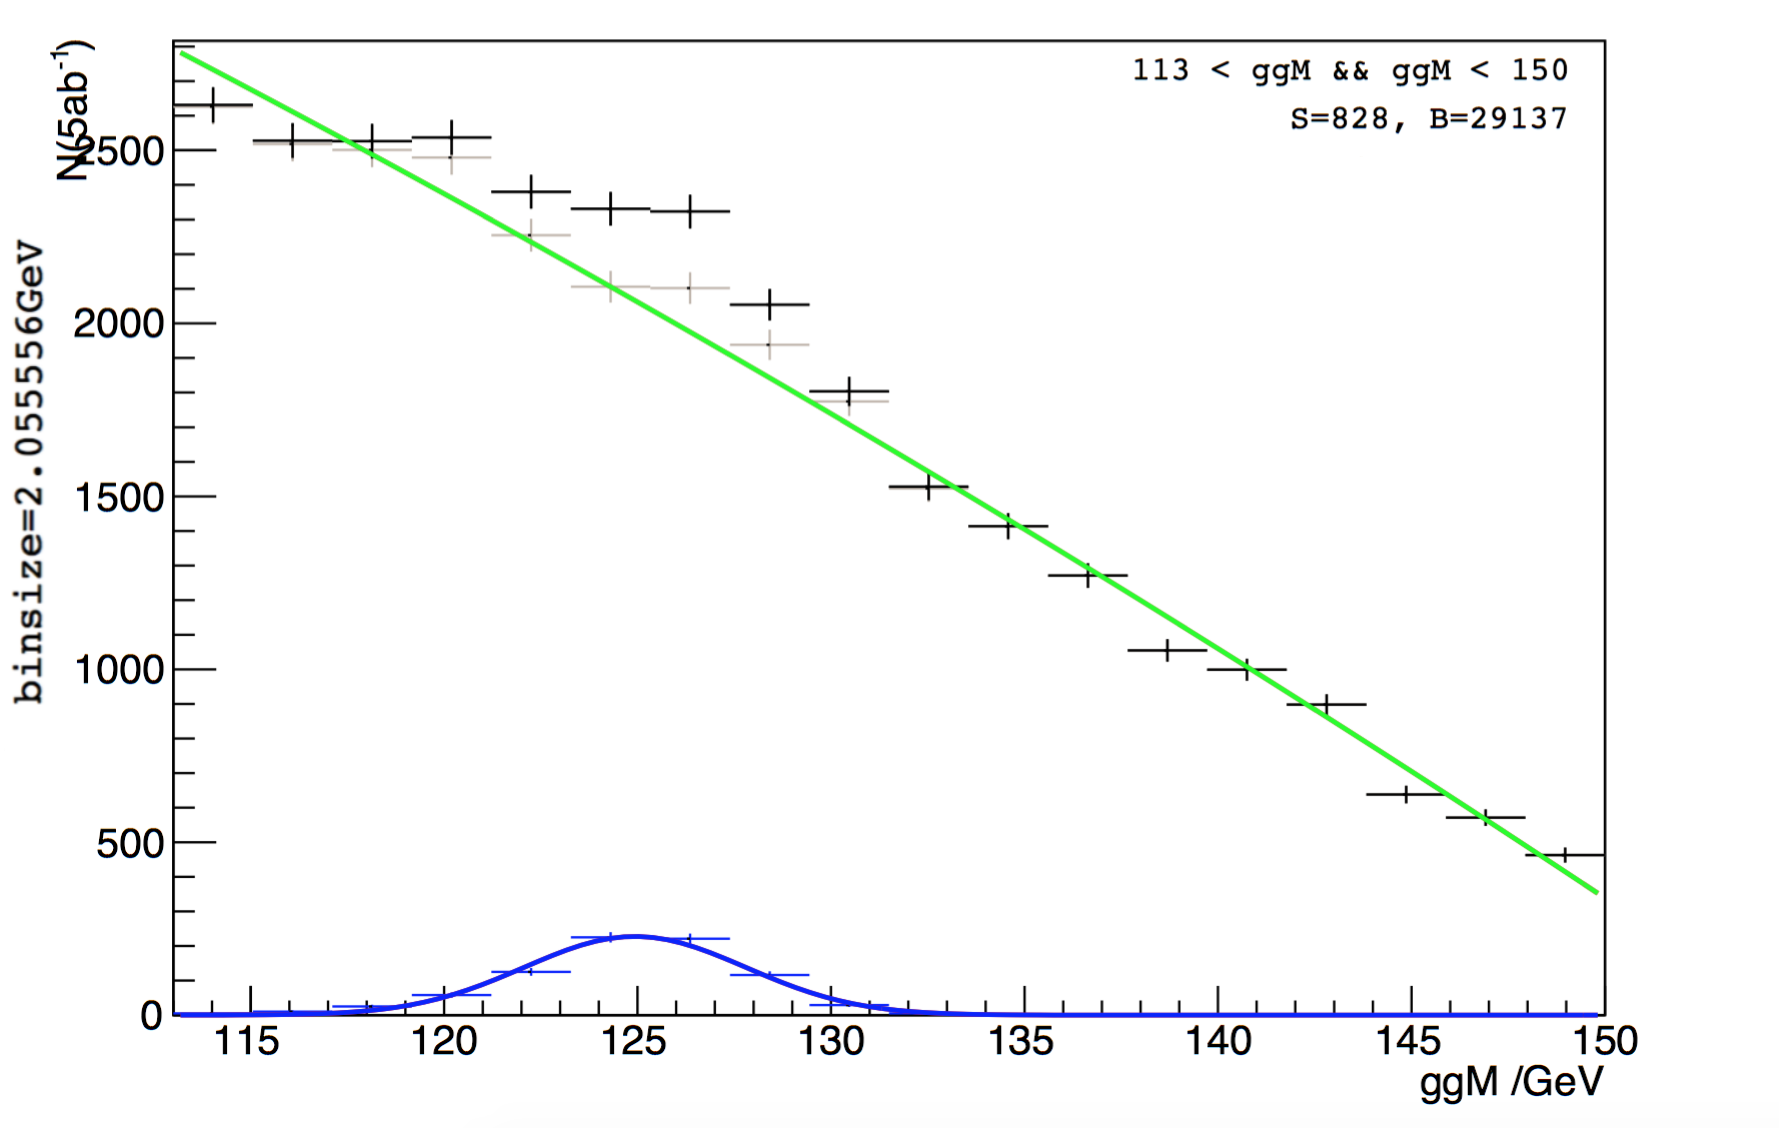
\includegraphics[width=0.6\textwidth]{ggM.png}
	\centering
	\caption{\textbf{Di-photon invariant mass distribution.} The blue line and green line are distributions fitted independently for signal and background distribution for MC evaluation of uncertainty.}
	\label{fig:ggM}
\end{figure}

\subsection{Evaluation of uncertainty}
In the actual experiment, we obtain a similar distribution after applying the cut chain and compare the distribution to this simulation based on the Standard Model. To obtain the signal event number, we apply a fit to the combined distribution of the signal and background events, and the uncertainty of the signal events comes from that of the fitting. Assuming we will obtain an (signal) distribution close to the Standard Model prediction, we can measure the uncertainty by attempting to perform a fitting on Monte Carlo generated distributions based on the given distribution. The background is relatively smooth, so a quadratic function is used as a fit function. The signal width comes mainly from the Ecal errors, and the actual Higgs width is obscured, so a simple Gaussian distribution is used. The fit to a distribution is done by the Minuit algorithm in the Root program (v6.04/16) \cite{root,minuit}, for two times, while the initial values are set close to the truth value. The uncertainty stabilizes as 10000 Monte Carlo distributions are fitted. The measurement is plotted in Fig. \ref{fig:N-DN} (a), and the uncertainty is 15.4\%. The uncertainty reported by the program is plotted in Fig. \ref{fig:N-DN}, with a mean value of 15.9\%, and an uncertainty of $\pm 0.06\%$. However, the mean value of the measurement systematically deviates from the truth value by about the 2.7\%, whose direct sum with the statistical uncertainty $15.4\%\oplus2.7\%\approx15.6$ (?) the reported uncertainty of $15.9\%$. Since the value of $\PRZH$ and $BR(\Zqq)$ is known precisely from electroweak precision measurement, the measured uncertainty of $BR(\Hgg)$ is simply that of $\qt$.

\begin{figure}[h]
	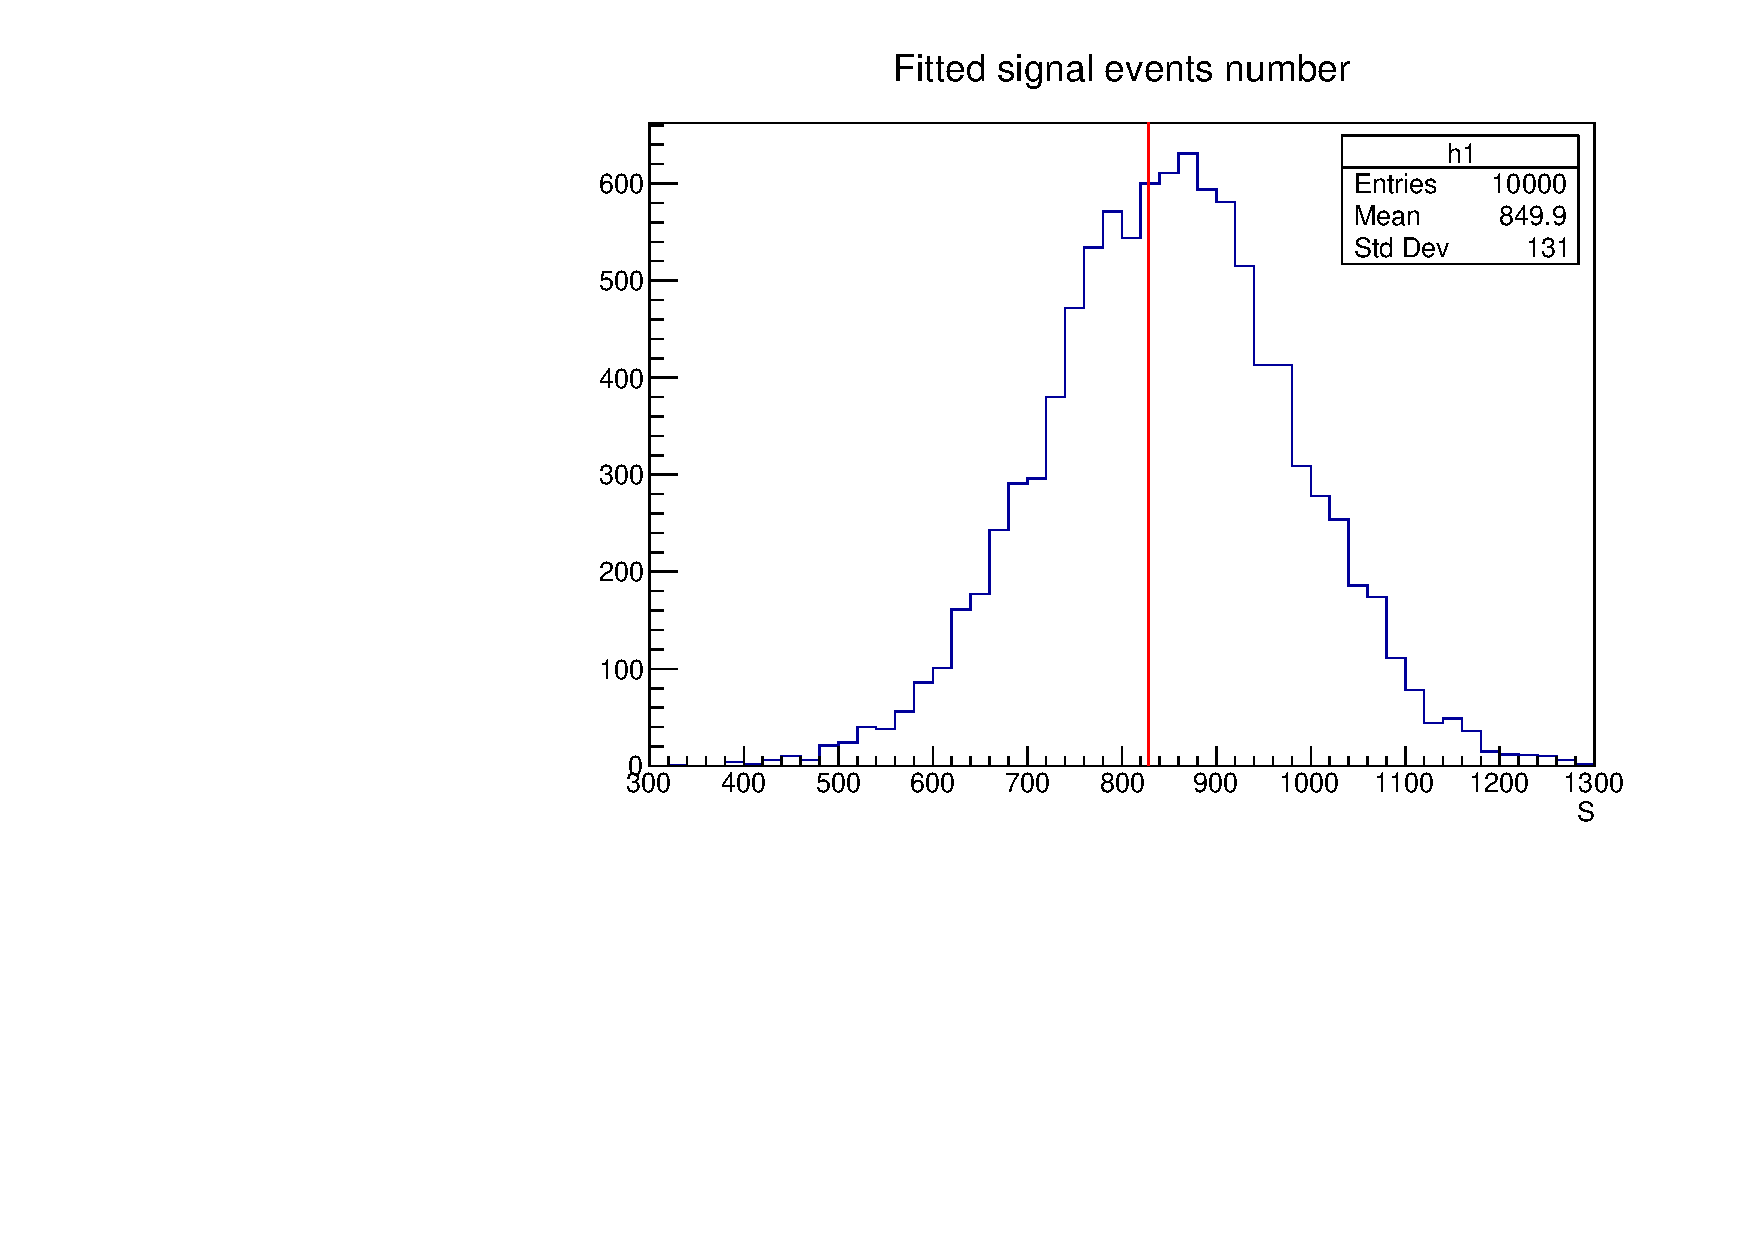
\includegraphics[scale=0.35,clip]{NFit.pdf}
	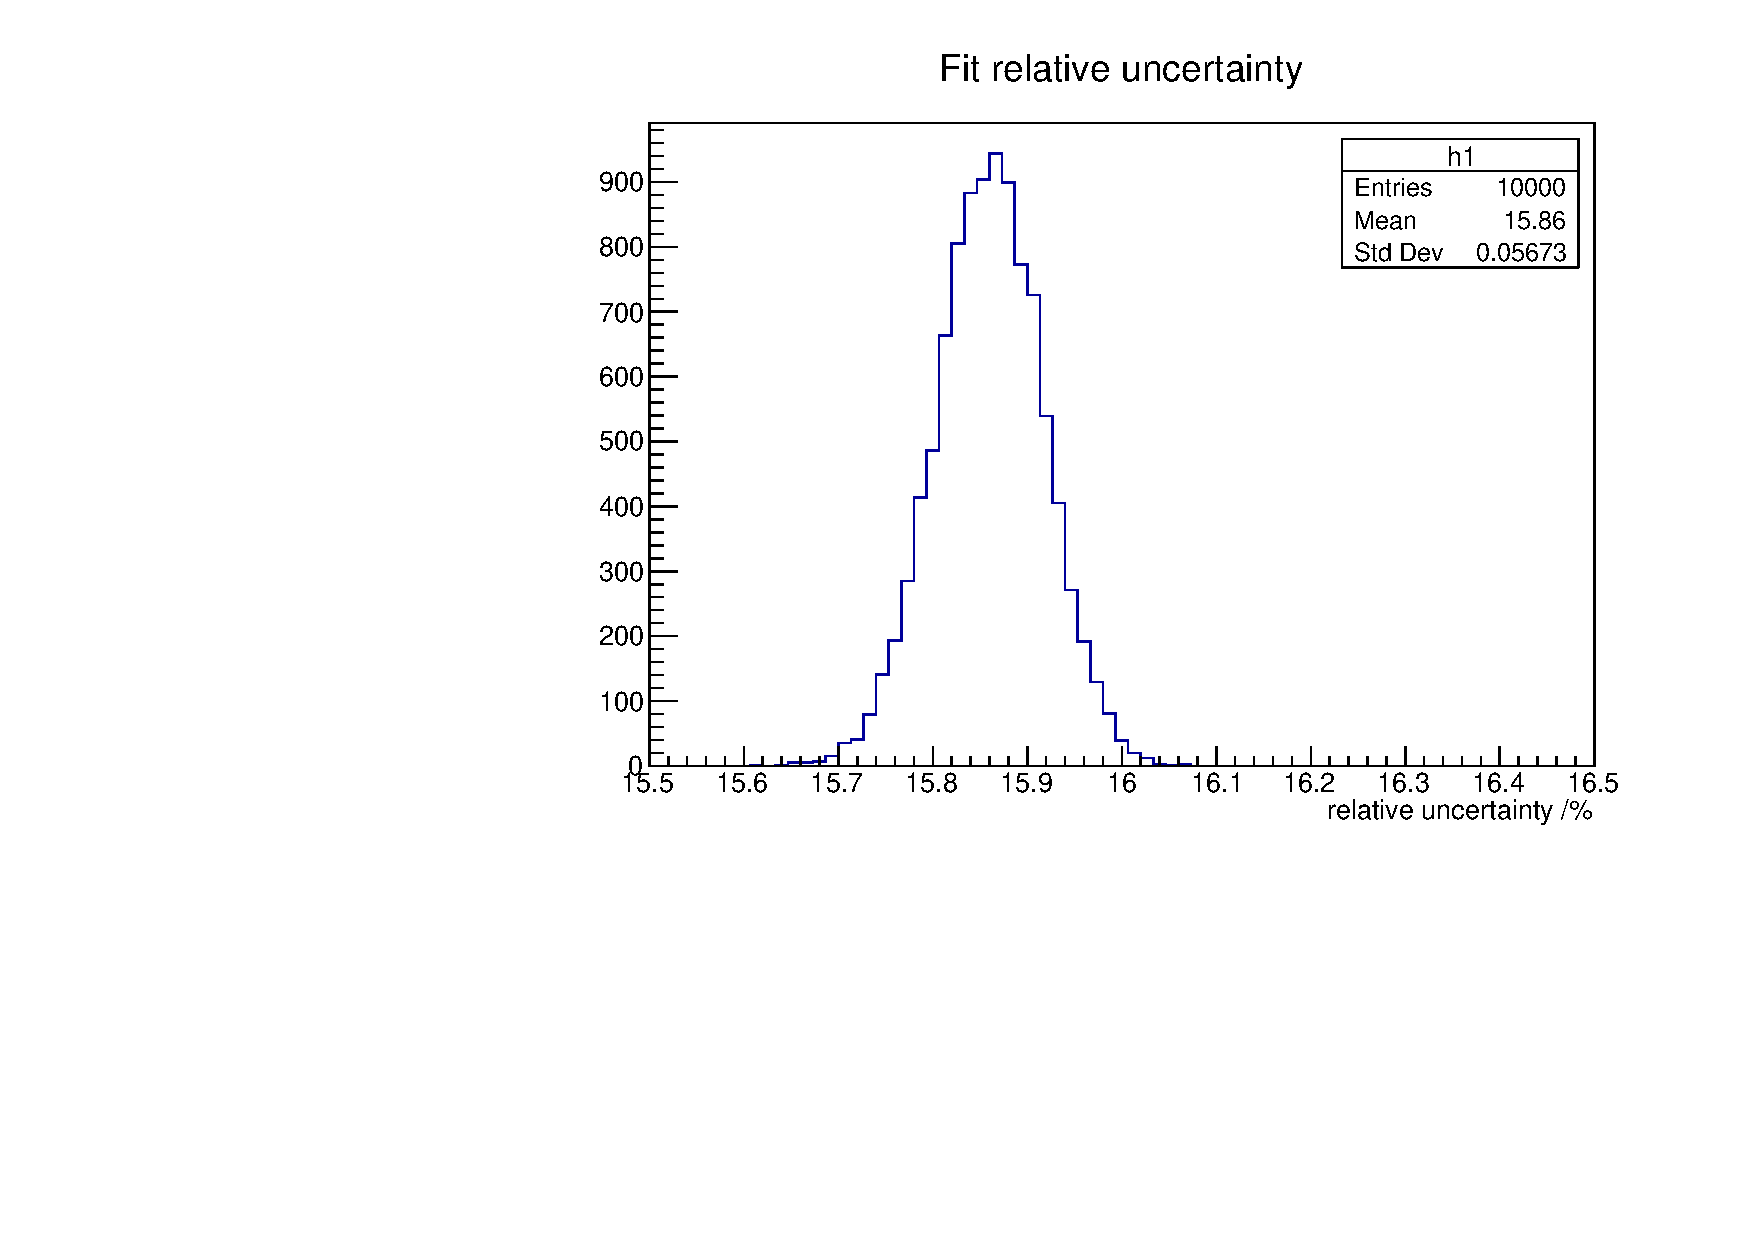
\includegraphics[scale=0.35,clip]{DNFit.pdf}
	\centering
	\caption{\textbf{Distribution of measurements and uncertainties in Monte Carlo simulation of the fitting.} (a) contains the expected signal count corresponding to the fit. The red line in (a) indicates the truth value. A uncertainty of 15.4\% can be achieved. (b) contains the fitting uncertainties (of the signal count) reported by the fitting program. The mean value 15.6\% is in agreement with the standard deviation of (a). The uncertainty of the measurement uncertainty is $\pm 0.06\%$. [Update!]}
	\label{fig:N-DN}
\end{figure}

\section{Relation to photo reconstruction algorithm}
\label{sec:photonrec}
We also study the dependence of our measurement's uncertainty on the photon conversion recovery algorithm and variance in signal width due to calorimeter performance. The photon recovery algorithm used in this paper boosts the total reconstruction success rate from 81\% to 92.5\% (in addition to some rare cases where $\gamma_1$ and $\gamma_2$ are reversed, i.e. the energy comparison is reversed in the full simulation due to calorimeter uncertainty, which are deemed unsuccessful here). We explore the dependence of $\delta s/s$ ($s=\qt$) on the efficiency of the photon recovery algorithm by simply compensating back or further deducting certain amount of expected signal events in the Monte Carlo evaluation of the uncertainty. Dependence on the Ecal performance is also studied. The signal width ($\sim 2.9\GeV$ in previous analysis) that principally originate from Ecal is related to the direct sum of the uncertainty of the energy of the resonate photons, each of which is described by $\frac{r\%}{\sqrt{E_i}}\cdot E_i$, where $r$ is the scaled relative uncertainty of the Ecal, and $E_i$ the energy of the respective photons. The total uncertainty is event-dependent, so we will simplify the picture and present the dependence of measurement uncertainty on the signal width. Fig. \ref{fig:uncertainty} shows the dependence of the uncertainty on the total reconstruction efficiency and the width of the signal distribution. It can be seen that uncertainty mildly decrease as the reconstruction efficiency grows. For signal width of about 2.9 GeV (as in previous analysis), the uncertainty can reach below 15\% with more photons successfully reconstructed. The dependence on the signal width is much larger, apparently. For the level of reconstruction efficiency in this analysis, the uncertainty ranges from about 25\% to below 10\% as the signal width varies from 5 GeV to 1 GeV.

\begin{figure}[h]
	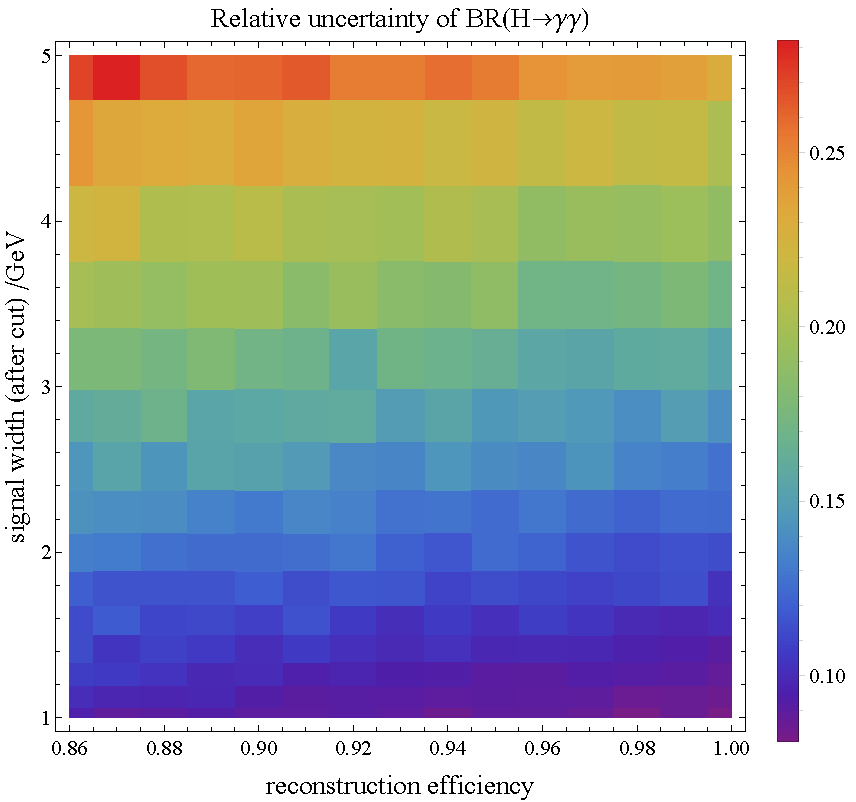
\includegraphics[scale=0.7,clip]{uncertainty.pdf}
	\centering
	\caption{\textbf{Dependence of relative uncertainty on total photon reconstruction efficiency and width of signal distribution.} Color represents relative uncertainty of the measurement $\delta s/s$, where $s=\qt$.}
	\label{fig:uncertainty}
\end{figure}

\bibliographystyle{cepcBibStyleWoTitle}
\bibliography{main}

\newpage
\appendix
\part*{Appendices}
\addcontentsline{toc}{part}{Appendices}
\section{Step-wise di-photon invariant mass distribution}
\begin{figure}[h]
	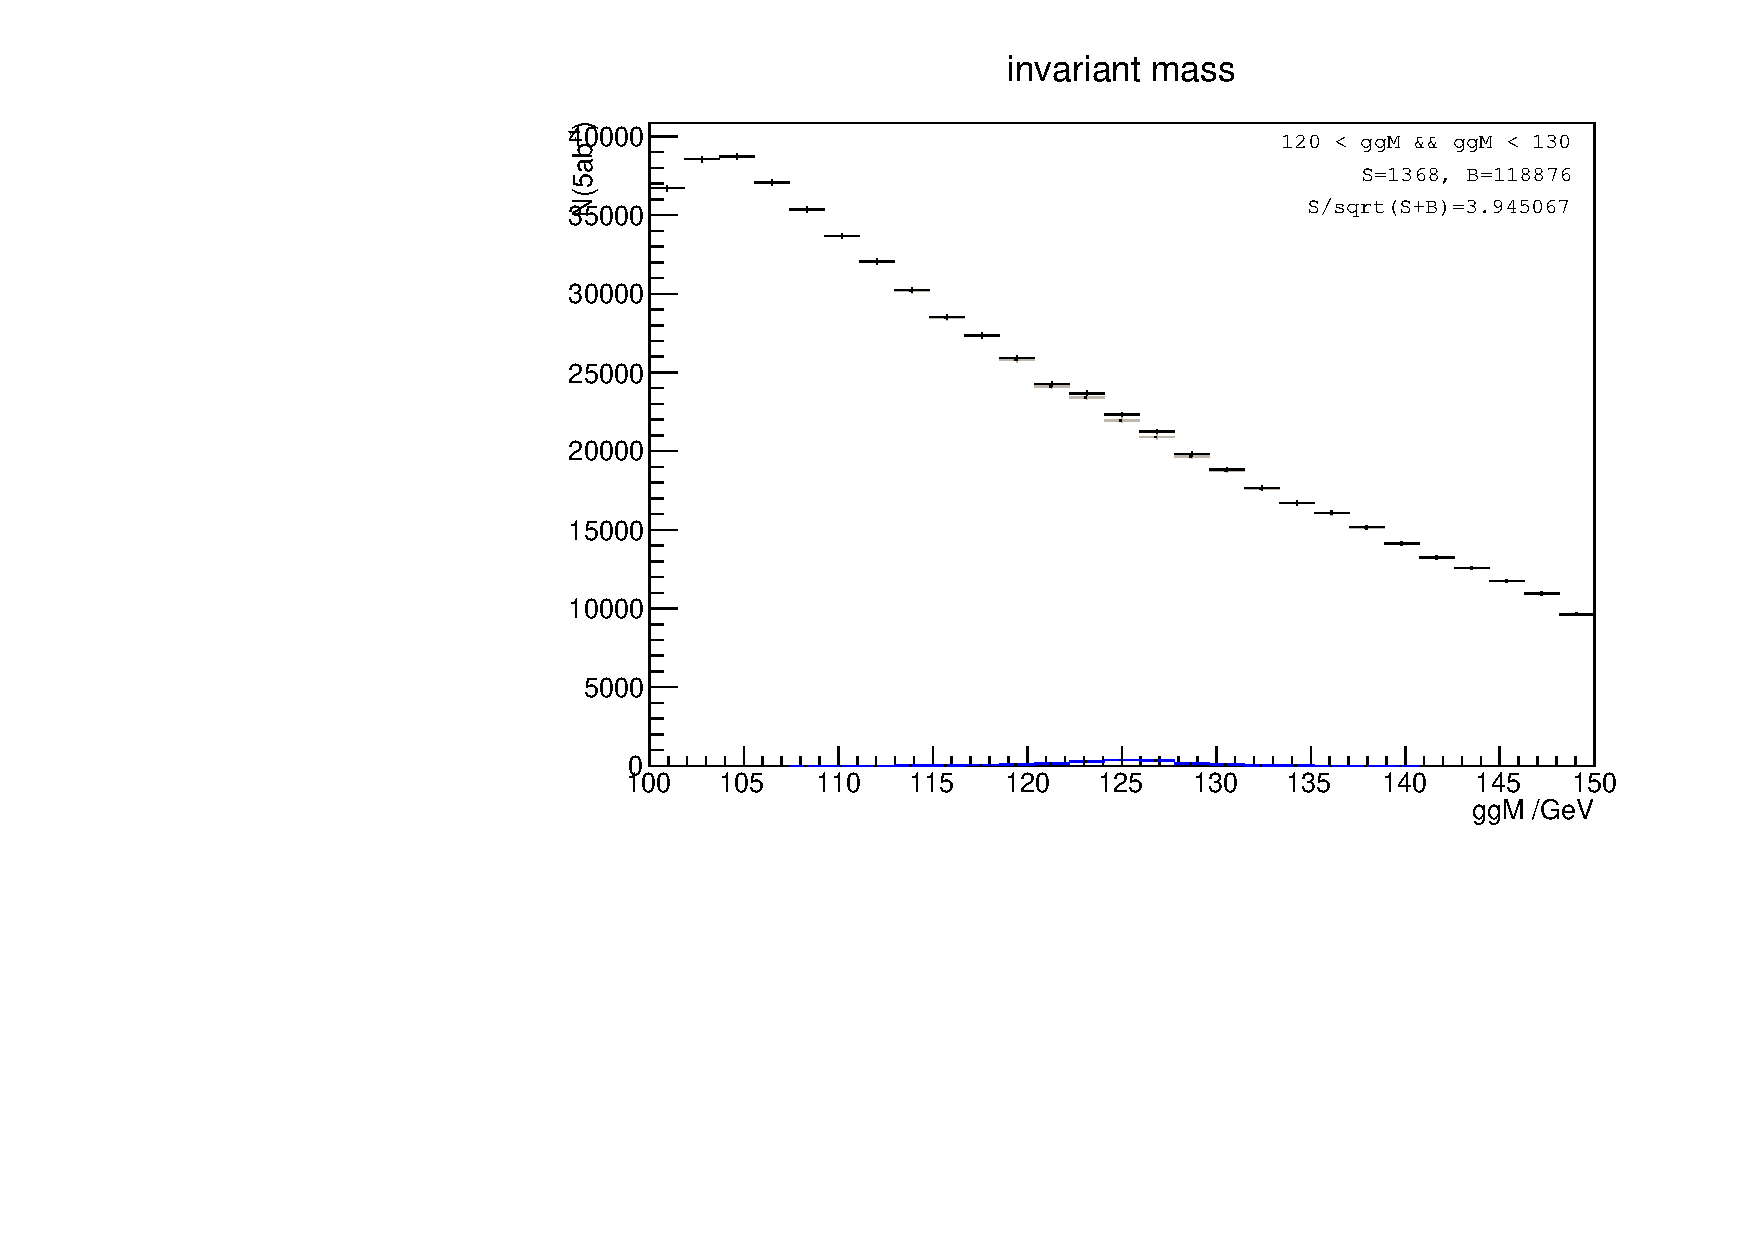
\includegraphics[scale=0.4,clip]{ggM_IIIXgd1.pdf}
	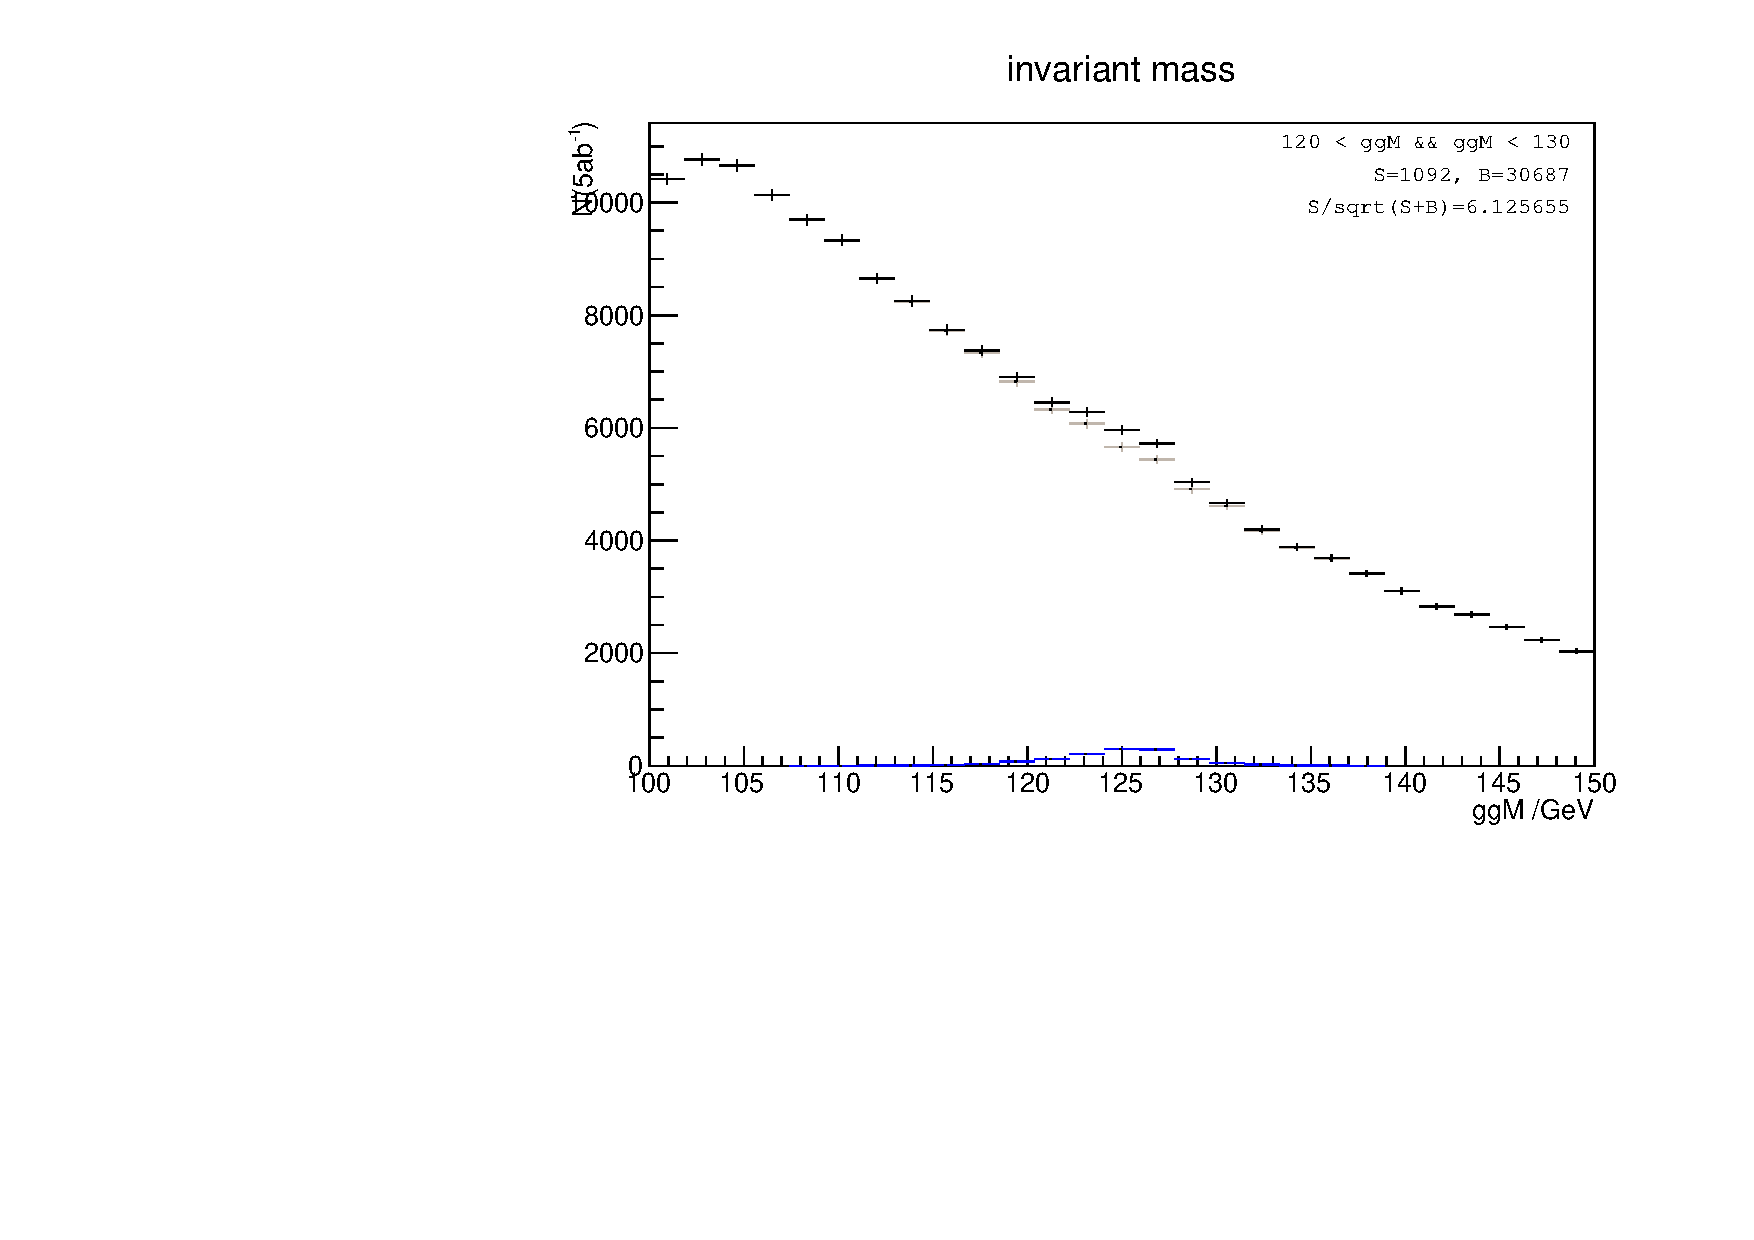
\includegraphics[scale=0.4,clip]{ggM_IIIXgd2.pdf}
	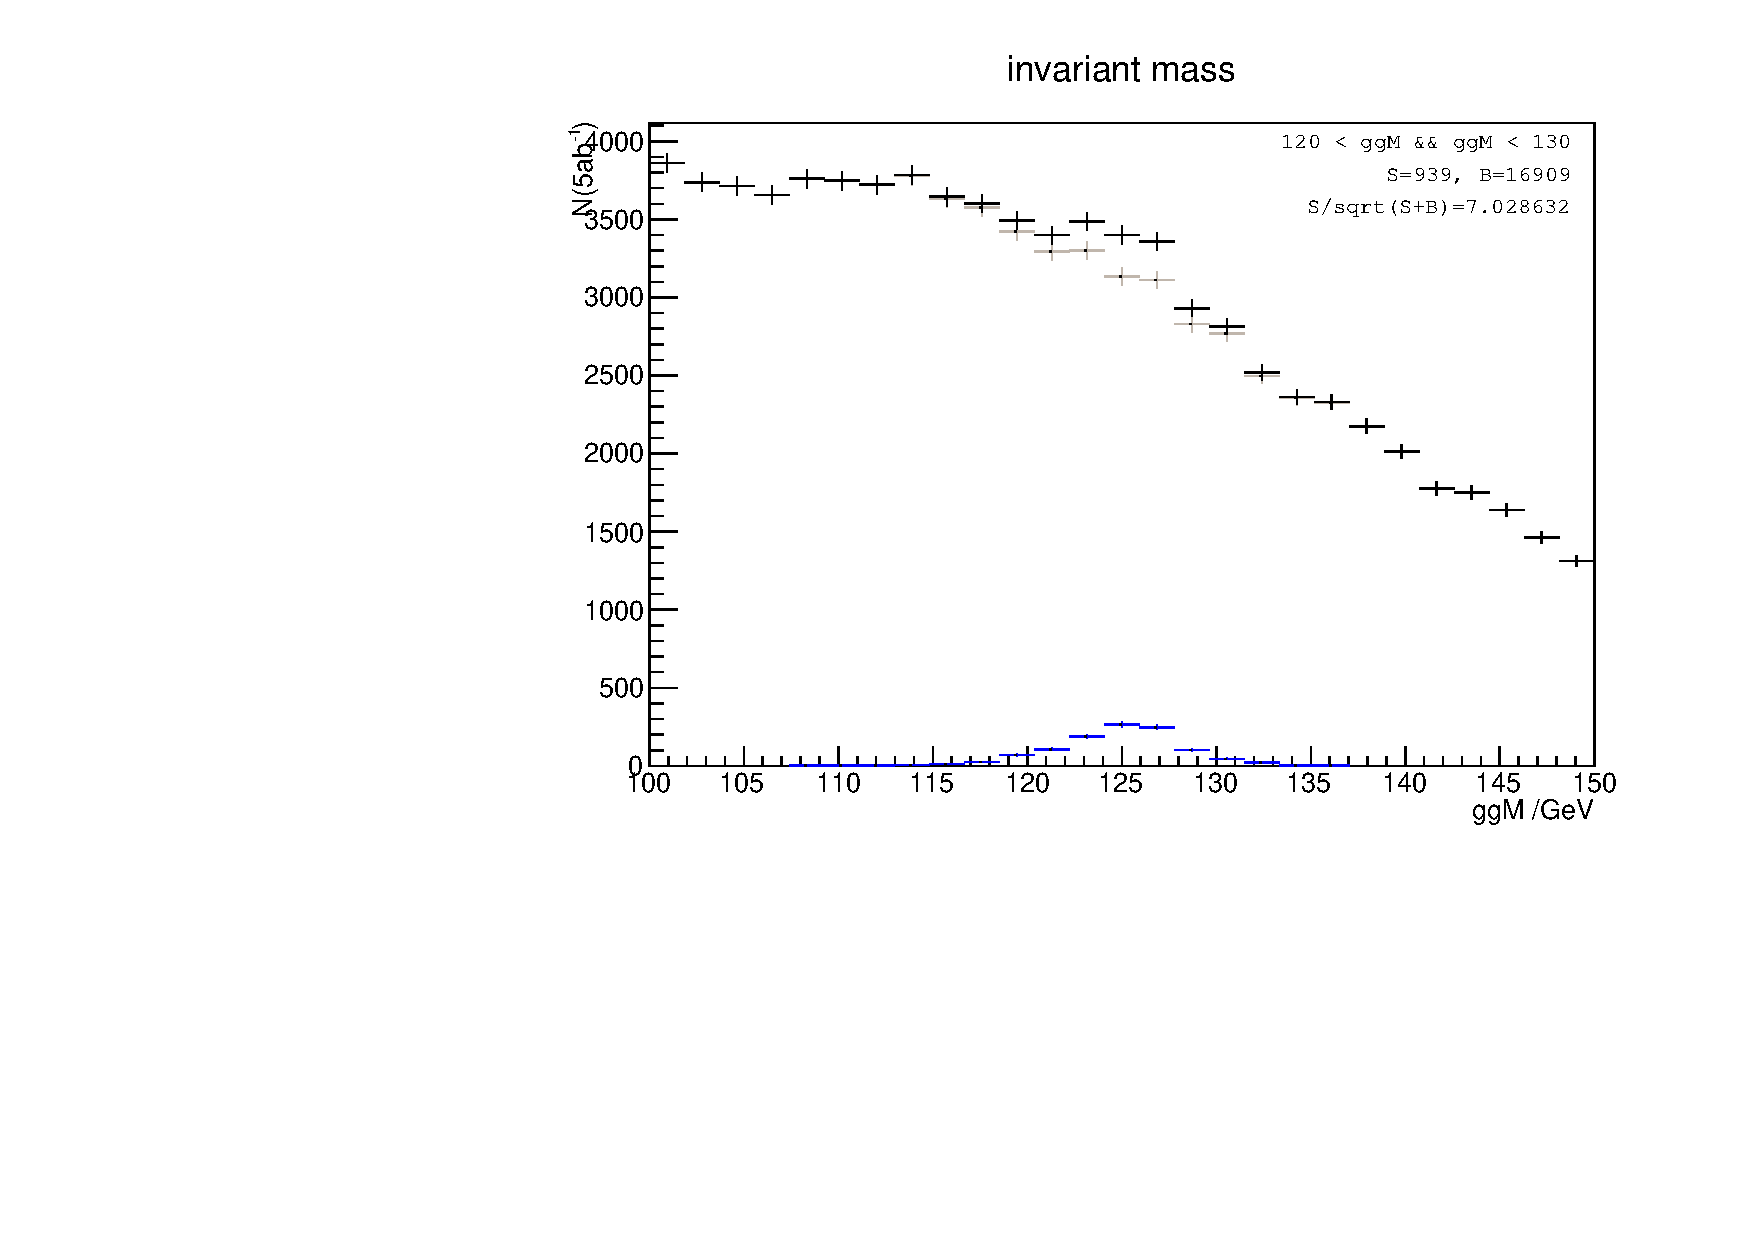
\includegraphics[scale=0.4,clip]{ggM_IIIXgd3.pdf}
	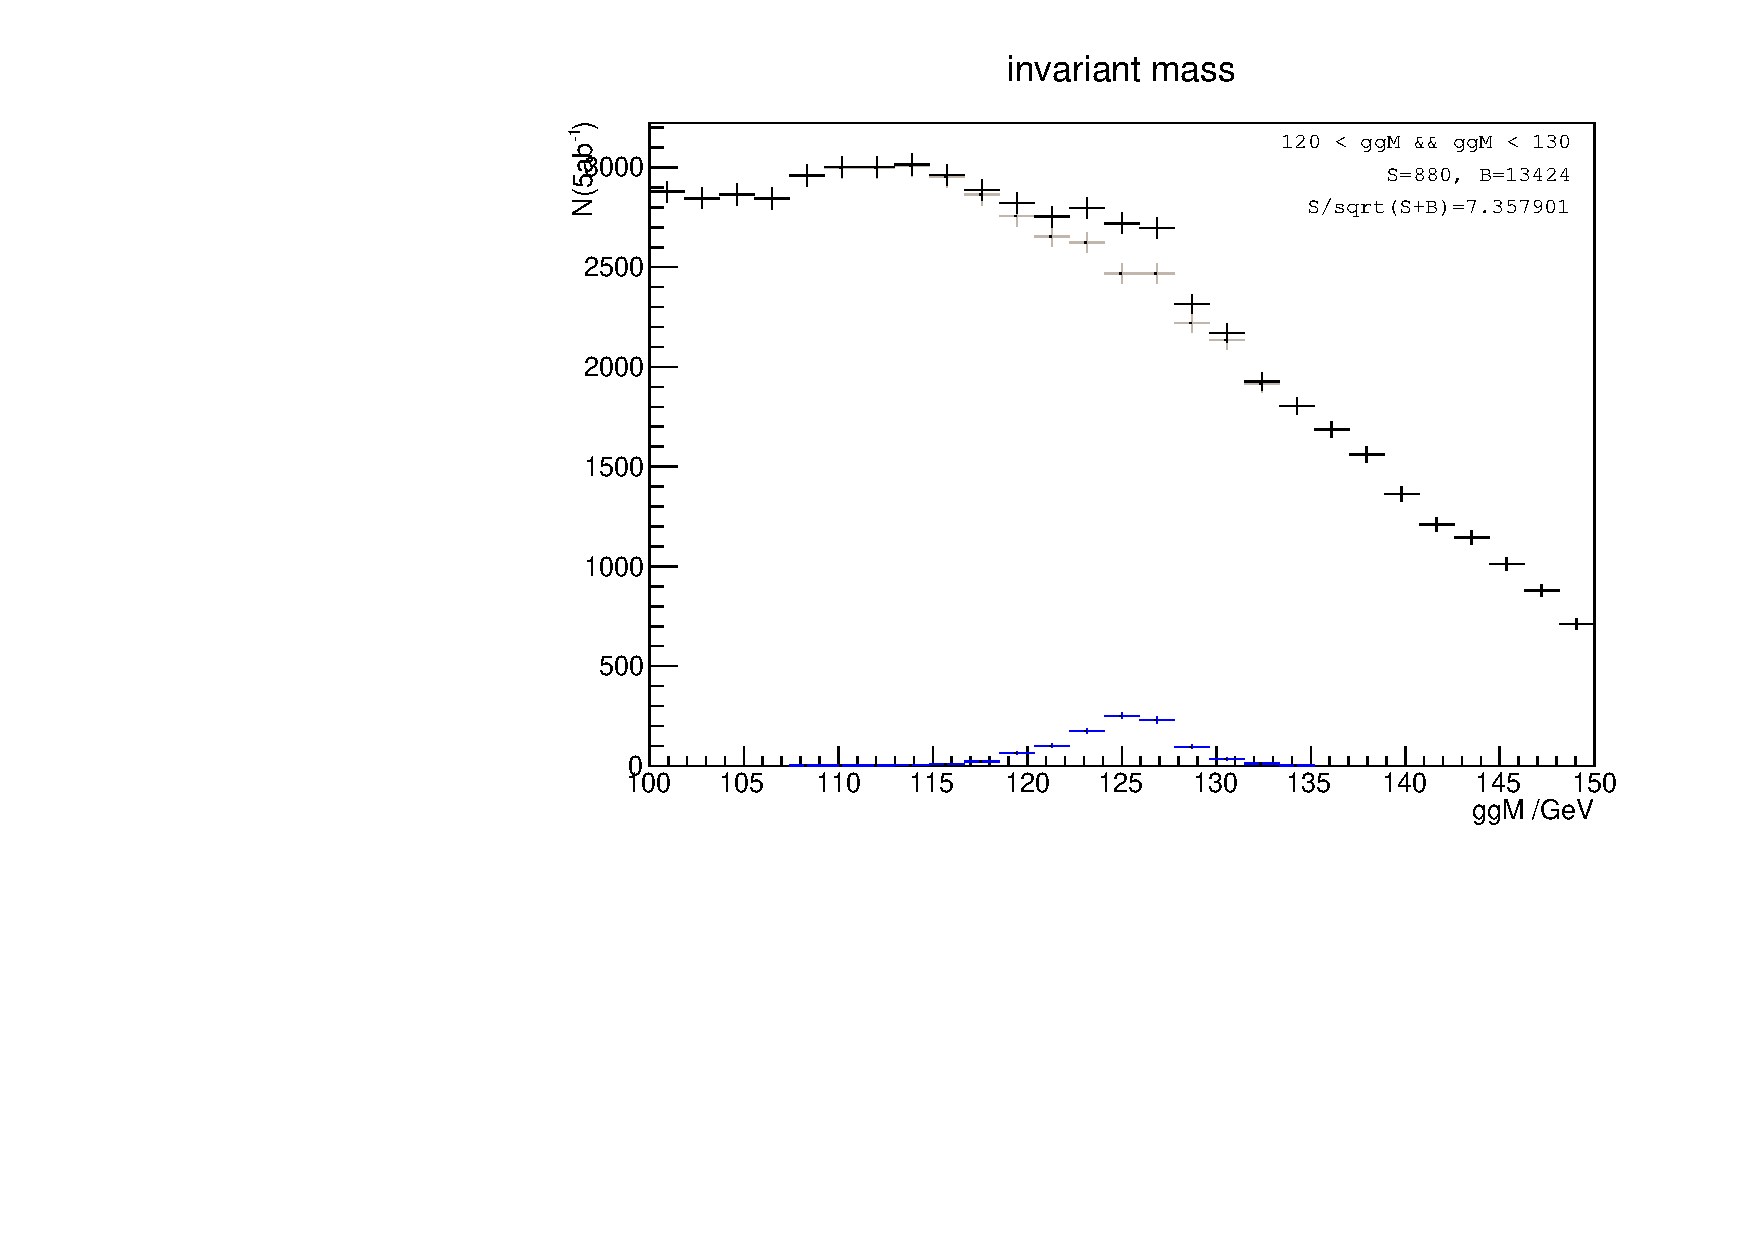
\includegraphics[scale=0.4,clip]{ggM_IIIXgd4.pdf}
	\caption{\textbf{Signal and background distribution in the di-photon invariant mass dimension}: after 1) Precut, 2) Cut1, 3) Cut2, 4) Cut3.}
	\label{fig:cuts_ggM}
\end{figure}
\end{document}
